\chapter{System}
Dieses Kapitel bietet eine grobe Übersicht über das ganze System, um die Zusammenhänge zwischen einzelnen Komponenten aufzuzeigen.
Auf einzelne Komponenten und Toolchains wird in den folgenden Kapiteln genauer eingegangen.


\section{Schematische Übersicht}
In Abbildung \ref{fig:UebersichtDebuggerToolchain} ist das ganze System abgebildet.
Das \textit{Zybo} beinhaltet neben dem FT2232-Chip auch noch diverse I/O-Peripherien, die in einer \textit{deep}-Applikation genutzt werden können.
Der FT2232 auf dem \textit{Zybo} übernimmt zwei verschiedene Funktionen.
Einerseits wird er als USB zu UART Brücke (schwarzer Pfeil) verwendet, damit man mit dem Windows PC einfach eine serielle Verbindung mit dem Prozessor aufbauen kann, andererseits fungiert er als Brücke zum blauen JTAG-Bus.
Das bedeutet, er erhält Befehle von der OpenOCD-Software über USB und übersetzt diese elektrisch und auch logisch für das JTAG Interface.
OpenOCD ist eine Software-Zwischenschicht die für den Debugger benötigt wird.

Auf dem \textit{Windows PC} wird die \textit{deep}-Applikation in Eclipse geschrieben, kompiliert und debuggt.
Plugins erweitern Eclipse um die notwendigen Funktionen, die für die Entwicklung von \textit{deep}-Applikationen notwendig sind.
In dieser Übersicht sind beide Debug Toolchains, die ''klassische'' Abatron-Toolchain und die neue OpenOCD-Toolchain, abgebildet.

Bei der \textit{Abatron-Toolchain} wird das \textit{Abatron BDI3000} mit dem \textit{abatronInterface}-Plugin über die rote TCP/IP-Verbindung angesprochen.
Das BDI kommuniziert dann über die blaue JTAG-Verbindung direkt mit dem Zynq-Chip.

Die grünen Pfeile zeigen den Kommunikationsweg für die neuen OpenOCD-Toolchains.
OpenOCD bildet zusammen mit der richtigen Hardware, hier ist es der FT2232-Chip, einen kompletten Debugger und ist somit eine Alternative zum BDI3000.
Die OpenOCD-Software stellt einen \textit{gdb}-Server und auch ein CLI (\textit{Command Line Interface}) zur Verfügung.
% referenz zu openOCDInterface
Das neue Eclipse-Plugin \textit{''OpenOCDInterface''} verwendet das CLI über den TCP/IP-Port 4444 (grüner Pfeil) und bildet so die \textit{CLI-OpenOCD-Toolchain}.
OpenOCD verwendet dann den \textit{WinUSB}-Treiber um mit dem FT2232-Chip über USB zu kommunizieren.
Der FT2232-Chip verwendet denselben blauen JTAG-Bus wie das BDI3000 zur Kommunikation mit dem Zynq.

Die \textit{gdb-OpenOCD-Toolchain} kann mit einem allein lauffähigen \textit{gdb} verwendet werden (orange, gestrichelter Pfeil), wie in Kapitel \ref{chapter:Der-gdb-Debugger} beschrieben.
Eine weitere Möglichkeit wäre ein \textit{gdb}-Plugin für Eclipse, damit der \textit{gdb} direkt aus Eclipse heraus verwendet werden kann.
Beide Varianten kommunizieren mit dem \textit{gdb}-Server von OpenOCD über den TCP/IP-Port 3333 (oranger Pfeil).


\begin{figure}[htbp]
	\centering
		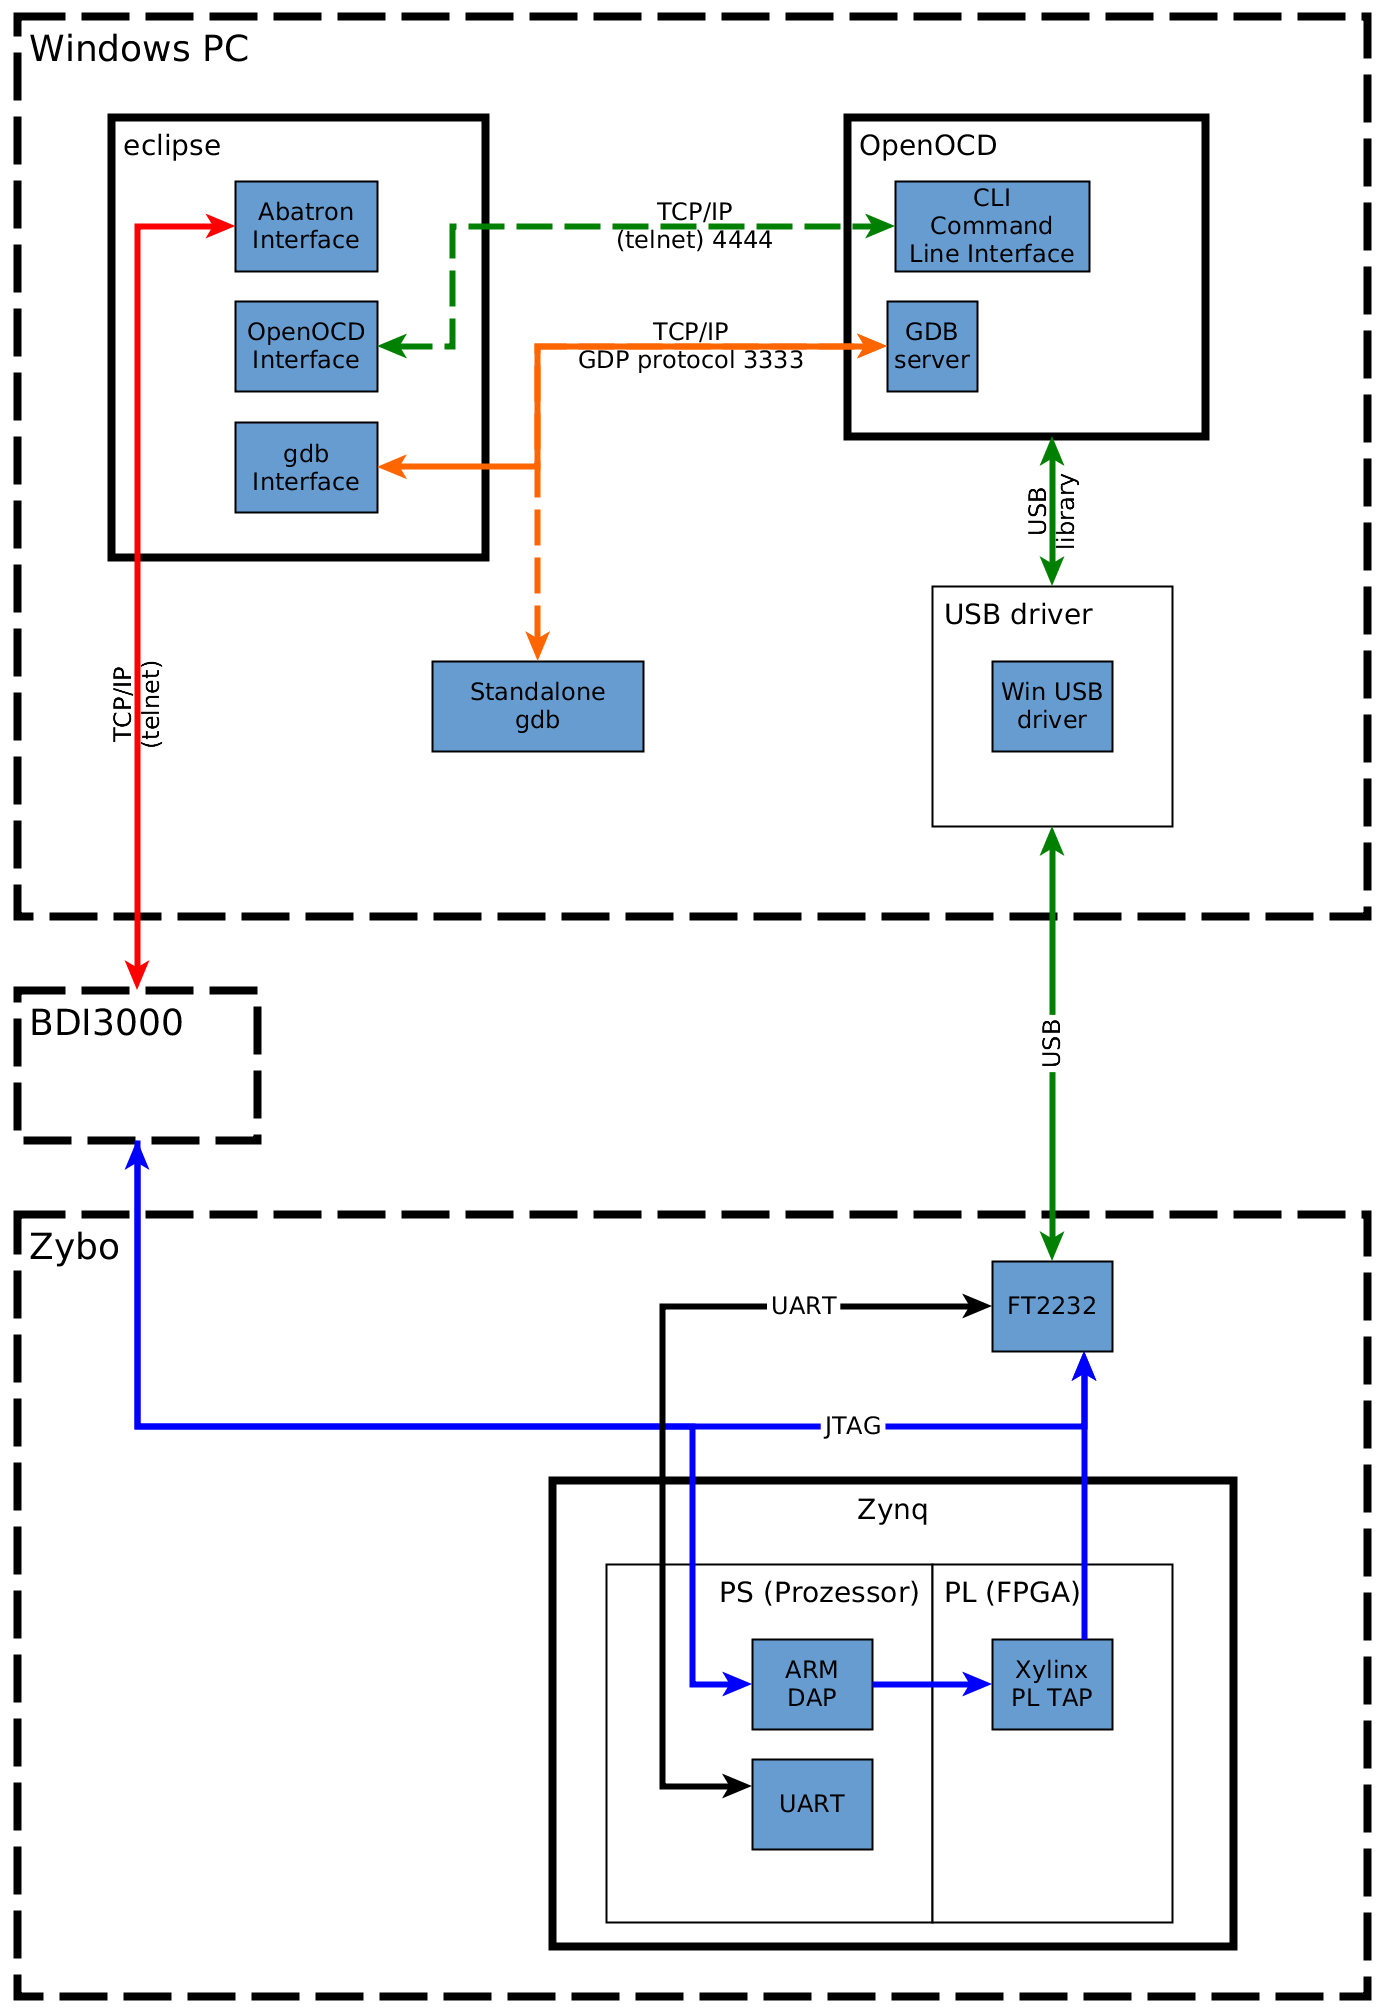
\includegraphics[width=\textwidth,height=\textheight,keepaspectratio]{graphs/embeddedDebuggerToolchain.png}
	\caption{Systemübersicht Debugger Toolchain}
	\label{fig:UebersichtDebuggerToolchain}
\end{figure}



\FloatBarrier
\section{Debugger Toolchains}
Im Folgenden werden die drei verschiedenen Toolchains genauer erklärt.

\subsection{Abatron-Toolchain}
Die \textit{Abatron-Toolchain} (Abbildung \ref{fig:AbatronToolchain}) benötigt weder die OpenOCD-Software noch den FT2232-Chip, dafür aber den teuren BDI3000-Debugger.
Diese ''klassische'' Toolchain nutzt das bestehende \textit{deep}-Plugin \textit{abatronInterface} und wird für die Entwicklung von \textit{deep} für den PowerPC verwendet.
In dieser Arbeit wird die \textit{Abatron-Toolchain} nicht verwendet.

\begin{figure}[htbp]
	\centering
		% 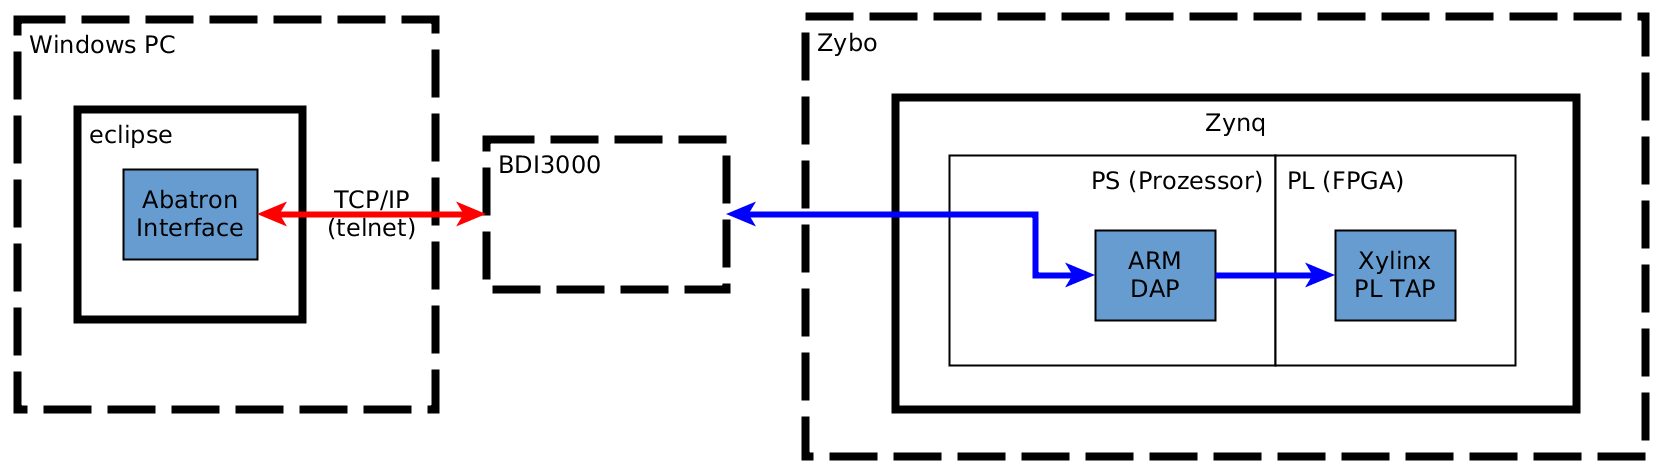
\includegraphics[width=\textwidth,height=\textheight,keepaspectratio]{graphs/abatronToolchain.png}
		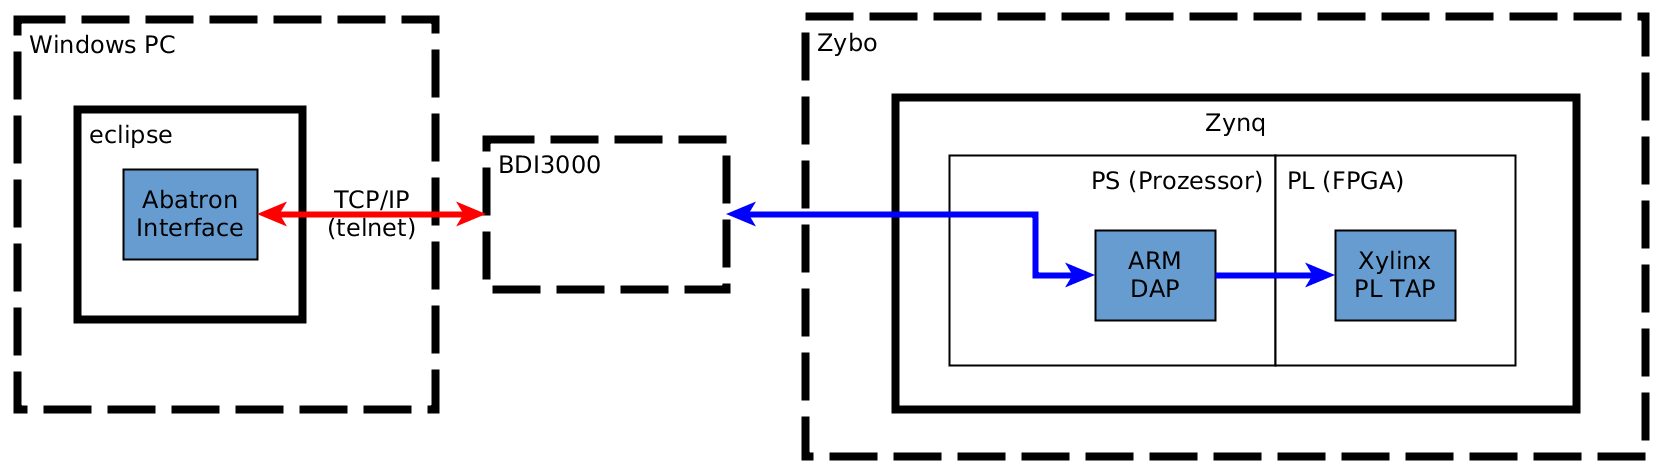
\includegraphics[width=10cm,height=\textheight,keepaspectratio]{graphs/abatronToolchain.png}
	\caption{Abatron-Toolchain}
	\label{fig:AbatronToolchain}
\end{figure}


\FloatBarrier
\subsection{CLI-OpenOCD-Toolchain}
Wie in Abbildung \ref{fig:CLIOpenOCDToolchain} zu sehen ist, wird das teure BDI wird für diese Toolchain nicht  benötigt.
% verbessern: satzbau
Da das CLI (Command Line Interface) von OpenOCD aber sehr ähnlich ist wie das CLI des BDI, ist eine Portierung der bestehenden \textit{Abatron-Toolchain} in die neue \textit{CLI-OpenOCD-Toolchain} relativ einfach.
Die \textit{CLI-OpenOCD-Toolchain} lehnt sich deshalb sehr stark an die bestehende \textit{Abatron-Toolchain} an.
% Die bestehende Toolchain für den PPC ist nicht auf der offiziellen \textit{deep}-Homepage dokumentiert.

Mit dieser Toolchain ist \textit{Sourcecode-Debugging} aber nicht möglich.
Das bedeutet, es ist nicht möglich im Sourcecode Breakpoints zu setzten oder durch einzelne Zeilen im Sourcecode zu steppen.
% TODO wirklich target commands?
Bestehende Möglichkeiten aus der alten \textit{Abatron-Toolchain}, wie \textit{Target Commands}, bleiben aber erhalten.
% TODO: Schema

Im Kapitel \ref{section:CLI-OpenOCD-Toolchain} wird die Implementation dieser Toolchain genauer beschrieben.


\begin{figure}[htbp]
	\centering
		% 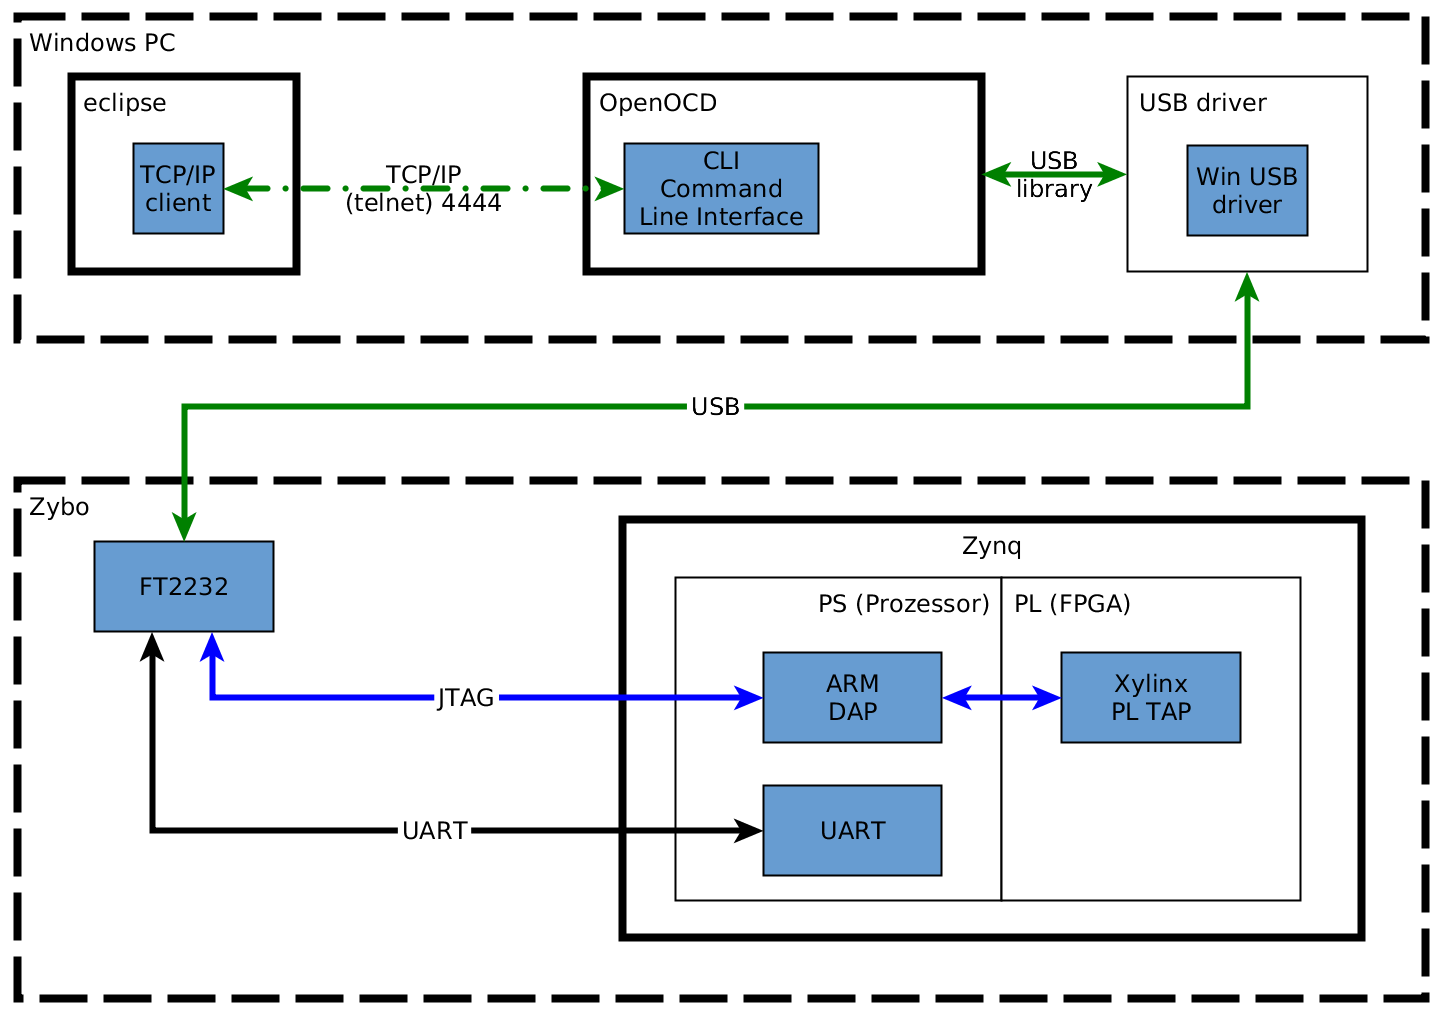
\includegraphics[width=\textwidth,height=\textheight,keepaspectratio]{graphs/CLIOpenOCDToolchain.png}
		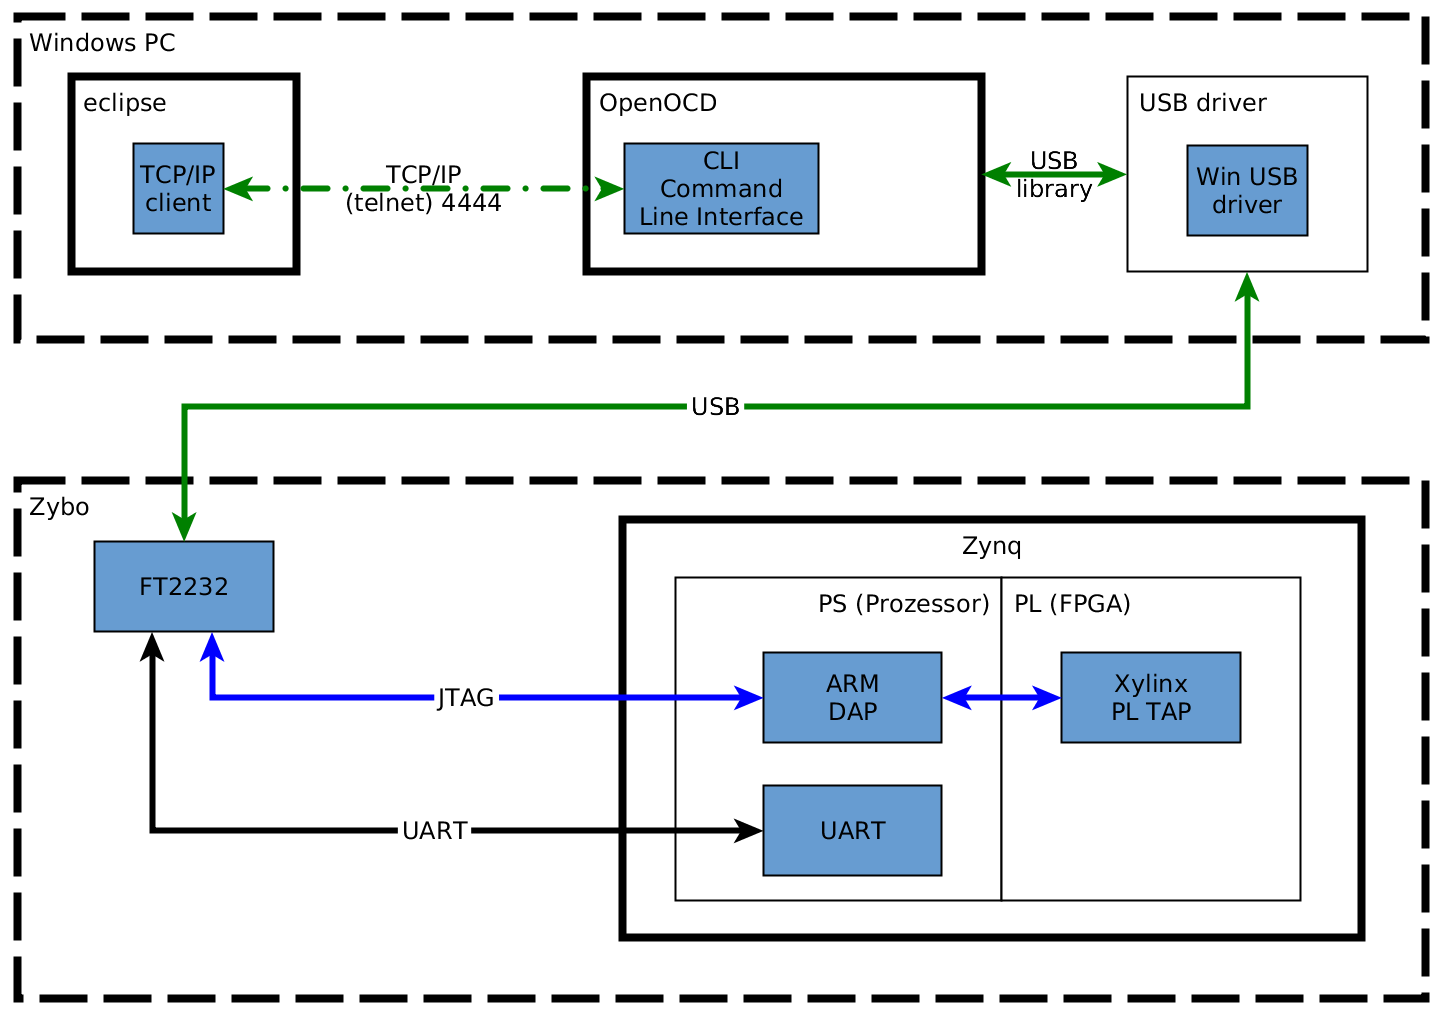
\includegraphics[width=10cm,height=\textheight,keepaspectratio]{graphs/CLIOpenOCDToolchain.png}
	\caption{CLI-OpenOCD-Toolchain}
	\label{fig:CLIOpenOCDToolchain}
\end{figure}


\FloatBarrier
\subsection{\textit{gdb}-OpenOCD-Toolchain}
In der \textit{gdb-OpenOCD-Toolchain} wird, wie bei der obigen Toolchain, ebenfalls die OpenOCD-Software und der FT2232-Chip verwendet.
Es wird aber nicht mehr ein Interface bestehend auf der ''klassischen'' Abatron Toolchain verwendet, sondern es wird direkt das CLI des \textit{gdb}-Debugger genutzt.
In der schematischen Übersicht der Toolchain in Abbildung \ref{fig:gdbOpenOCDToolchain} wird deutlich, dass sie fast die gleichen Komponenten nutzt wie die \textit{CLI-OpenOCD-Toolchain}.
% Dadurch kann \textit{Sourcecode-Debugging} direkt in Eclipse eingesetzt werden.
Mit dem \textit{gdb} können auch erweiterte Debugging-Featurers wie \textit{Sourcecode-Lookup} und \textit{Breakpoints} verwendet werden.
% günstige hardware

% TODO besserer text:
In dieser Arbeit wird nur die vereinfachte Toolchain mit dem standalone \textit{gdb}-Debugger implementiert.
Mit der vereinfachten Toolchain kann das CLI des \textit{gdb} in Kombination mit der \textit{OpenOCD-Toolchain} für zum Debuggen genutzt werden.

Die komplette \textit{gdb-OpenOCD-Toolchain} kann auf dieser Toolchain aufbauen.
Bei der kompletten \textit{gdb-OpenOCD-Toolchain} soll der \textit{gdb} im Eclipse integriert werden.
Dadurch kann in Eclipse die Applikation entwickelt und auch debuggt werden.

Im Kapitel \ref{chapter:Der-gdb-Debugger} wird diese Toolchain detailliert beschrieben.


\begin{figure}[htbp]
	\centering
		% 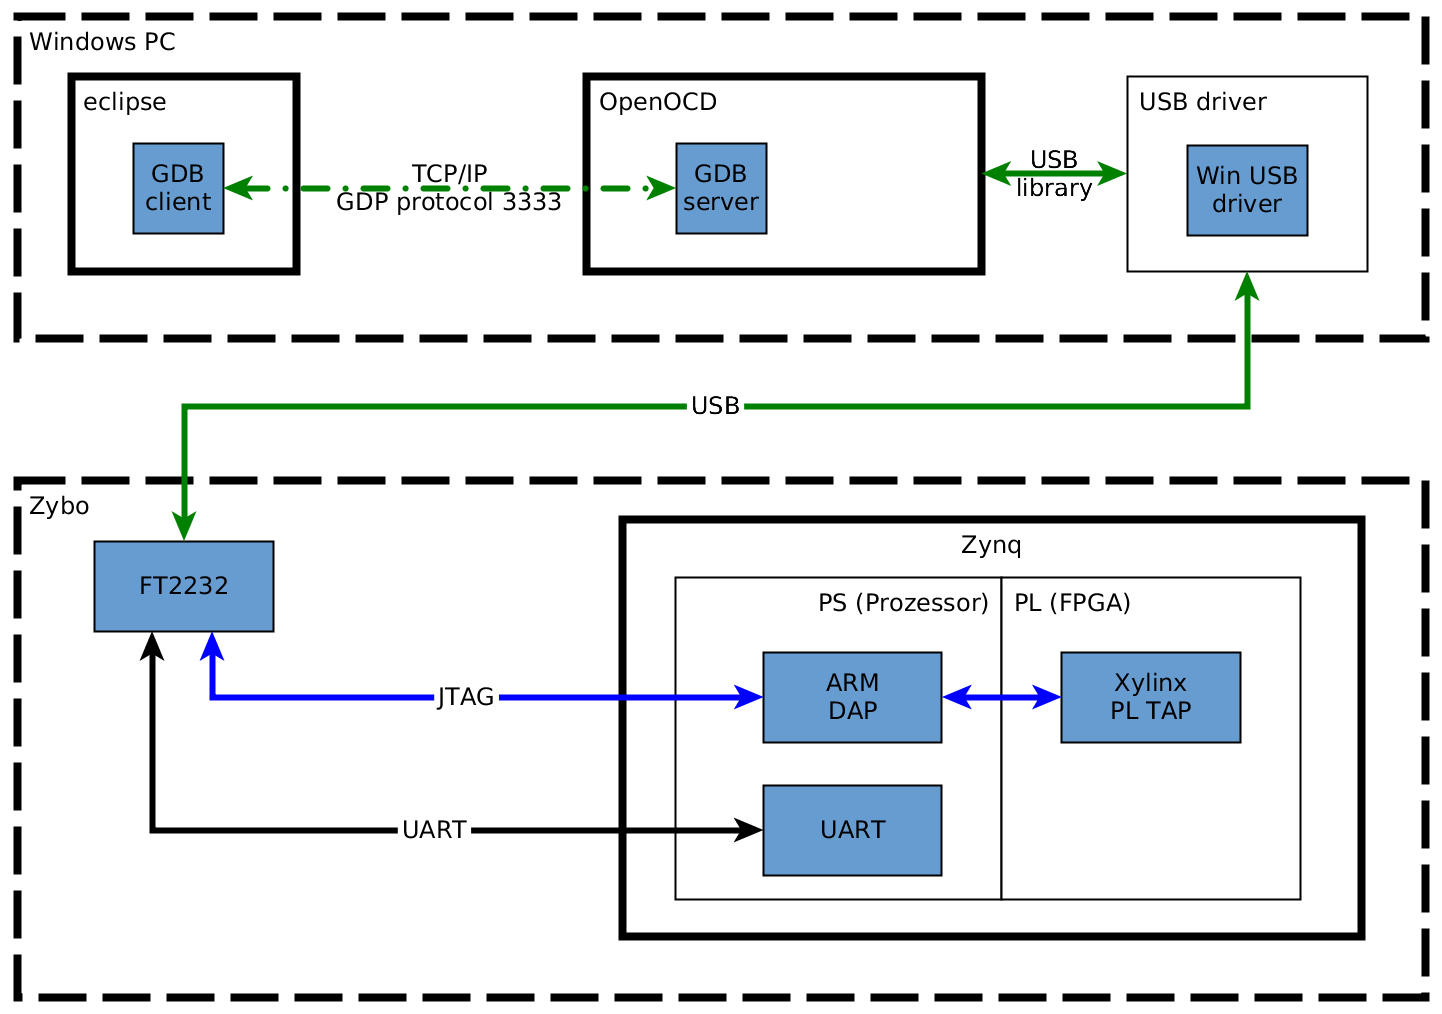
\includegraphics[width=\textwidth,height=\textheight,keepaspectratio]{graphs/gdbOpenOCDToolchain.png}
		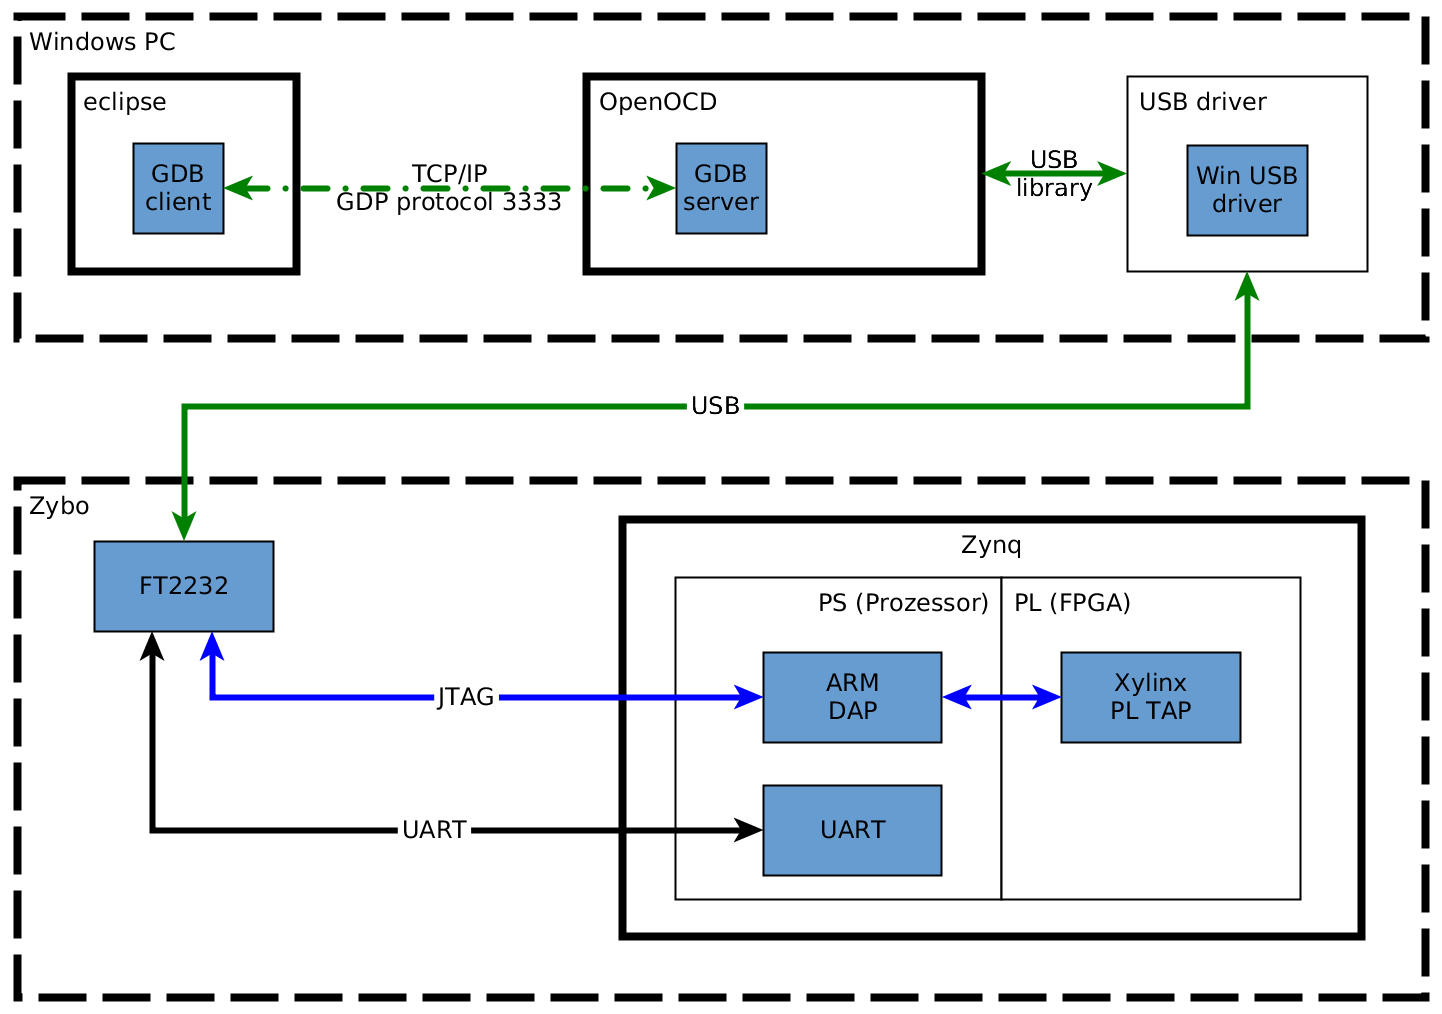
\includegraphics[width=10cm,height=\textheight,keepaspectratio]{graphs/gdbOpenOCDToolchain.png}
	\caption{\textit{gdb}-OpenOCD-Toolchain}
	\label{fig:gdbOpenOCDToolchain}
\end{figure}